\section{Materials and parts lists}\label{sec:appendix-a}

\subsection{Floating platform}

The floating platform is built from the following parts:

\begin{itemize}
  \item 1 main baffle made from 22~mm glulam. The front bumper,
    servo and containing straps for the batteries are screwed to this baffle. (Blueprints in \cref{fig:appendix-blueprint-main-plate}.)
  \item 4 floating elements made from 70~mm XPS cell foam. (Blueprint in \cref{fig:appendix-blueprint-ponton}.)
  \item 2 boards that goes below the floating elements, and stabilize them (Blueprint in \cref{fig:appendix-blueprint-ponton}.)
  \item 4 250~mm M10 stainless steel threaded rods
  \item 8 70~mm M6 stainless steel threaded rods
  \item 4 M10 nuts
  \item 4 M10 lock nuts
  \item 16 M6 nuts
  \item 8 M6 wing nuts
  \item 8 M10 washers
  \item A 20~mm plastic tube bent to a quarter circle with a radius of 400~mm
  \item 2 straps to keep the batteries in place
  \item 4 handles
  \item Self drilling screws and washers used to attach electronics, battery
    straps, and the bumper.
\end{itemize}

\subsection{Electronics}\label{sec:appendix-electronics}
The electronic components mounted on the platform are:
\begin{itemize}
  \item 1 Arduino Leonardo
  \item 1 Dual VNH5019 Motor Driver Shield
  \item 2 2725 Brushless out-runner motors 1600~kv
  \item 2 ESC which matches the brushless motors
  \item 2 plastic propellers
  \item 1 15~kg torque servo
  \item 1 R9D Radio Control Receiver
  \item 1 blue power-LED (mounted on the cover)
  \item 1 220~$\Omega$ resistor
  \item 1 power switch (mounted on the cover)
  \item 1 0.1 $\mu$F capacitor rated for at least 12~V \footnote{\label{fotnot_app} These parts can be replaced with any suitable 12~V to 5~V power supply.}
  \item 1 22 $\mu$F capacitor rated for at least 5~V\textsuperscript{\ref{fotnot_app}}
  \item 1 L4940V5 linear regulator\textsuperscript{\ref{fotnot_app}}
  \item Protoboard for the 5~V PSU\textsuperscript{\ref{fotnot_app}} (See schematic \cref{fig:appendix-circuit-diagrams} in \cref{sec:appendix-b}.)
  \item A few meters unshielded main cable 2x1.50~mm$^2$
  \item A few meters signal cable
  \item A few sensor cables and connectors (for servo, ESC, and power to RC receiver)
  \item Heat-shrink tubing to cover connections
  \item A few blade receptacle 4.8x0.5~mm fully insulated, blade terminal red
    4.8x0.8~mm, ring cable lug 4.3~mm used to connect the cables together.
  \item A few 2.54~mm pin headers for the connections to the Arduino.
\end{itemize}
 \Cref{fig:appendix-circuit-diagrams} in \cref{sec:appendix-b} shows the complete circuit diagram of these parts. The electronics are connected according to the circuit diagrams, and the files in \texttt{RBR\_driver.zip} is loaded onto the Arduino.

\subsection{RBR modules}
Each of the two RBR modules are built from the following parts:
\begin{itemize}
  \item 1 top baffle made from a 22~mm glulam (\cref{fig:appendix-blueprint-rbr-module})
  \item 1 bottom baffle made from a 22~mm thick glulam (\cref{fig:appendix-blueprint-rbr-module})
  \item 1 3D printed motor mount
  \item 1 motor, shuck, and gearbox taken from a Meec Tools 12~VDC cordless drill 
  \item 3 330~mm M10 stainless steel threaded rods
  \item 3 M10 locking nuts
  \item 9 M10 nuts
  \item 12 M10 washers
  \item 2 50~mm M4 stainless steel threaded rods
  \item 2 110~mm M4 stainless steel threaded rods
  \item 10 M4 washers
  \item 10 M4 nuts
  \item 4 long M3 screws
  \item 4 M3 nuts
  \item 4 M3 washers
  \item 1 shaft guide NS29
  \item 1 piece of 50~mm wide and 200~mm long piece of 2~mm stainless steel
    bent to form a wave baffle.
  \item 1 piece of metal to put pressure on top of the motor.
\end{itemize}

\subsection{Covers for RBR modules and electronics}
The cover for the RBR module is made from 5 pieces of 3~mm thick acrylic glass
glued together, with a handle attached on top. The blueprints for these are shown in
\cref{fig:appendix-blueprint-rbr-cover} and \cref{fig:appendix-blueprint-electronic-cover},
both in \cref{sec:appendix-b}.

The cover for the electronics are made from 13 pieces of 3~mm thick acrylic glass
glued together. On top of this cover the power switch is connected. This cover
was fastened to the platform using handmade angle brackets and a nut.

\clearpage
\section{Blueprints and schematics}\label{sec:appendix-b}
\subsection{Circuit diagrams}
\begin{figure}[H]
  \centering
  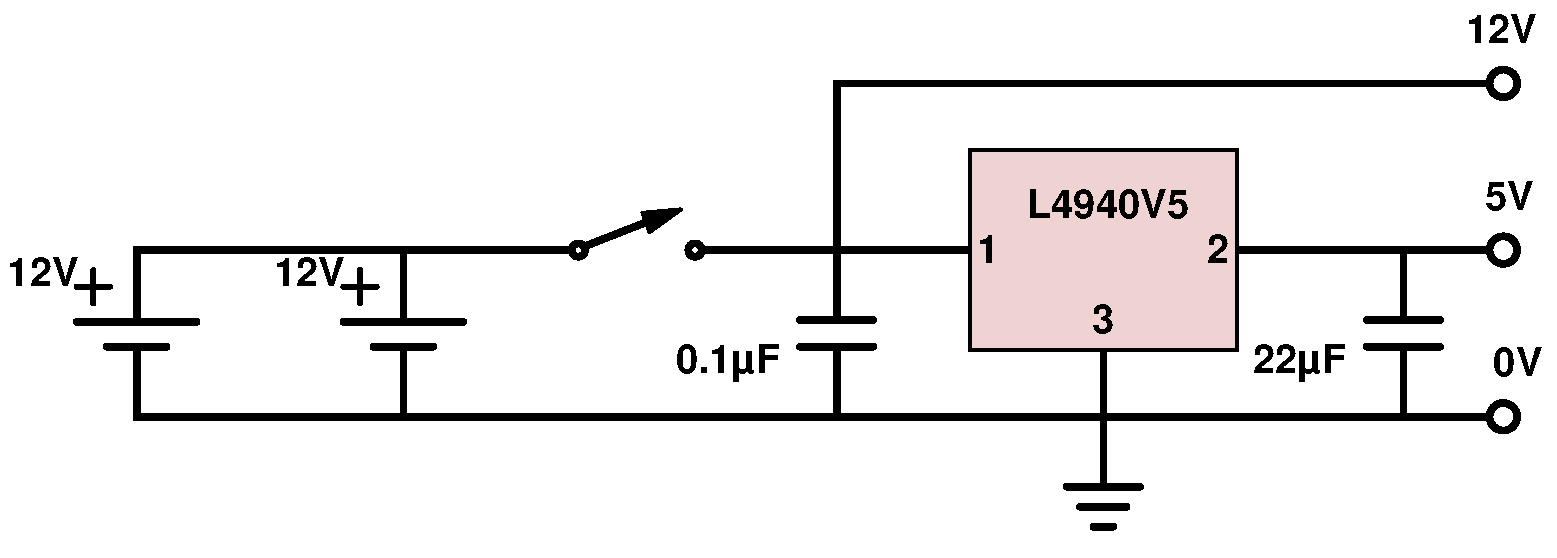
\includegraphics[width=0.7\textwidth]{Powersupply}
  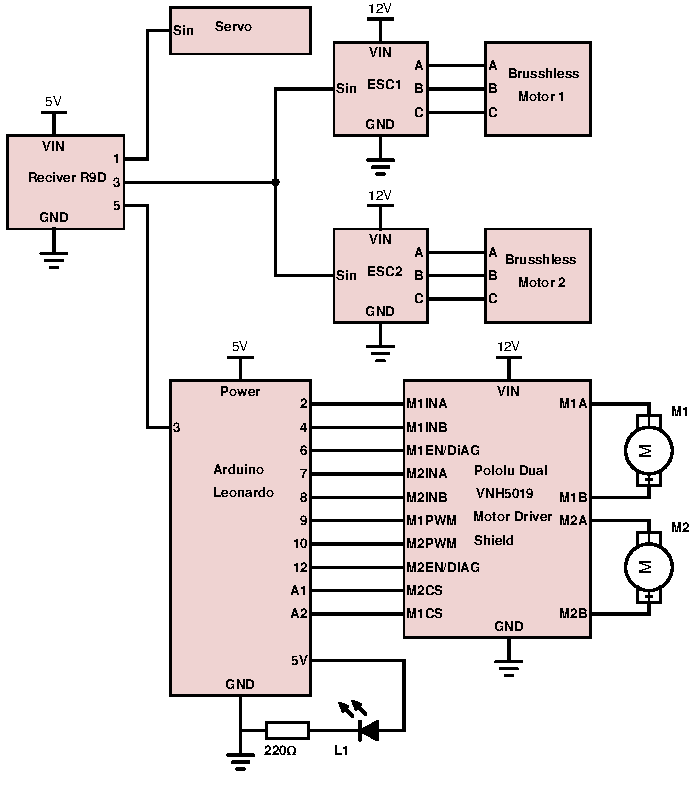
\includegraphics[width=0.7\textwidth]{circuit}
  \caption{The circuit diagram for the electronics.}
  \label{fig:appendix-circuit-diagrams}
\end{figure}

\clearpage
\subsection{Covers}
\begin{figure}[H]
  \centering
  \raisebox{-\height}{ 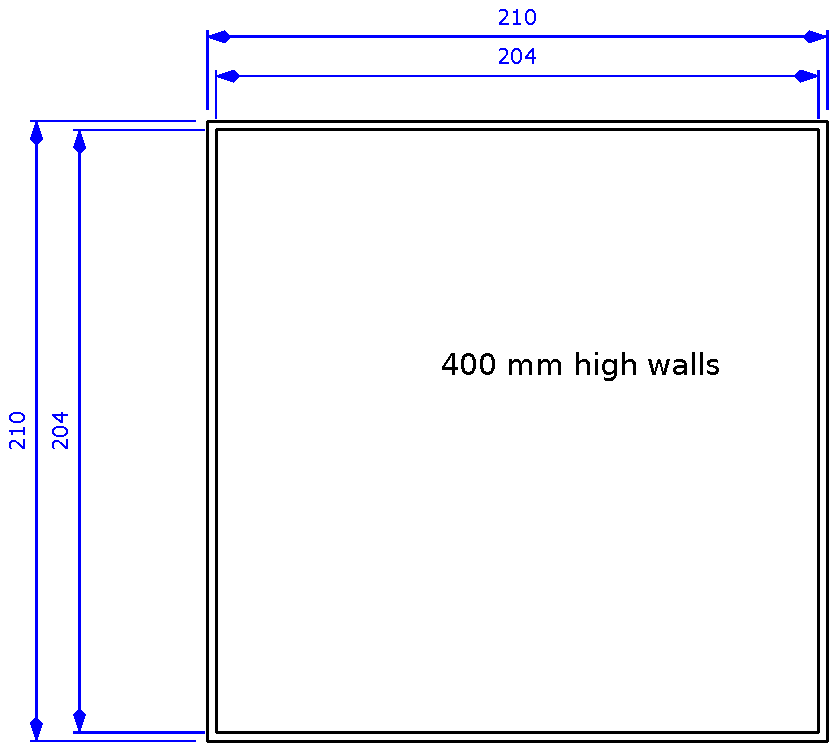
\includegraphics[scale=1]{RBR_cover}}
  \caption{Blueprint of the RBR cover in scale 1:2.}
  \label{fig:appendix-blueprint-rbr-cover}
\end{figure}

\begin{figure}[H]
  \centering
  \raisebox{-\height}{ 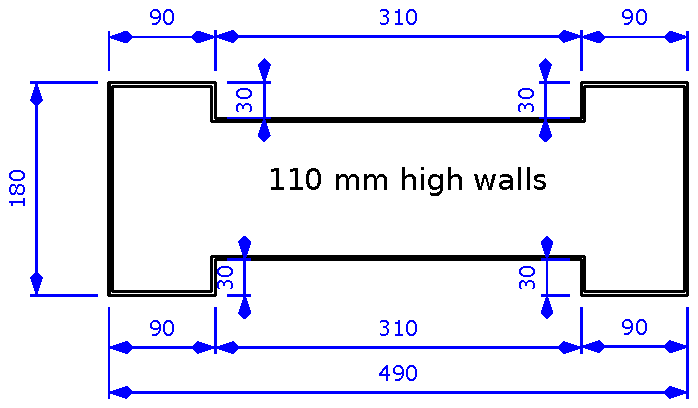
\includegraphics[scale=1]{Electric_cover}}
  \caption{Blueprint of the electric cover in scale 1:5.}
  \label{fig:appendix-blueprint-electronic-cover}
\end{figure}

\clearpage
\subsection{Blueprints}
\begin{figure}[H]
  \centering
   \raisebox{-\height}{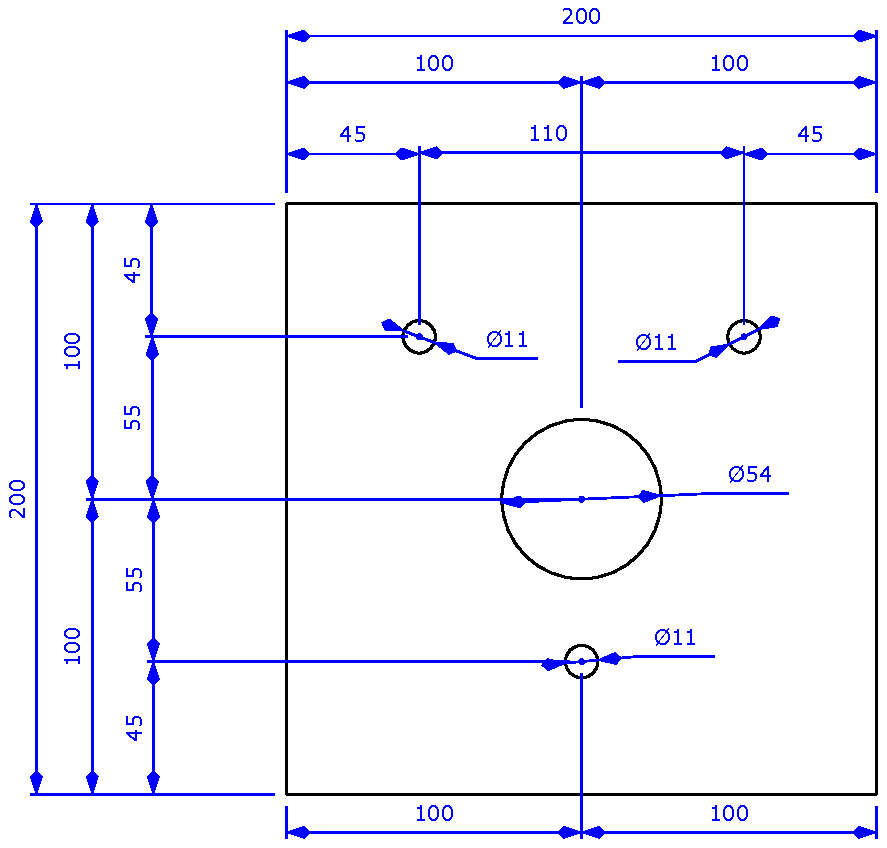
\includegraphics[scale=0.4]{RBR_mod_Top}}
   \raisebox{-1.02\height}{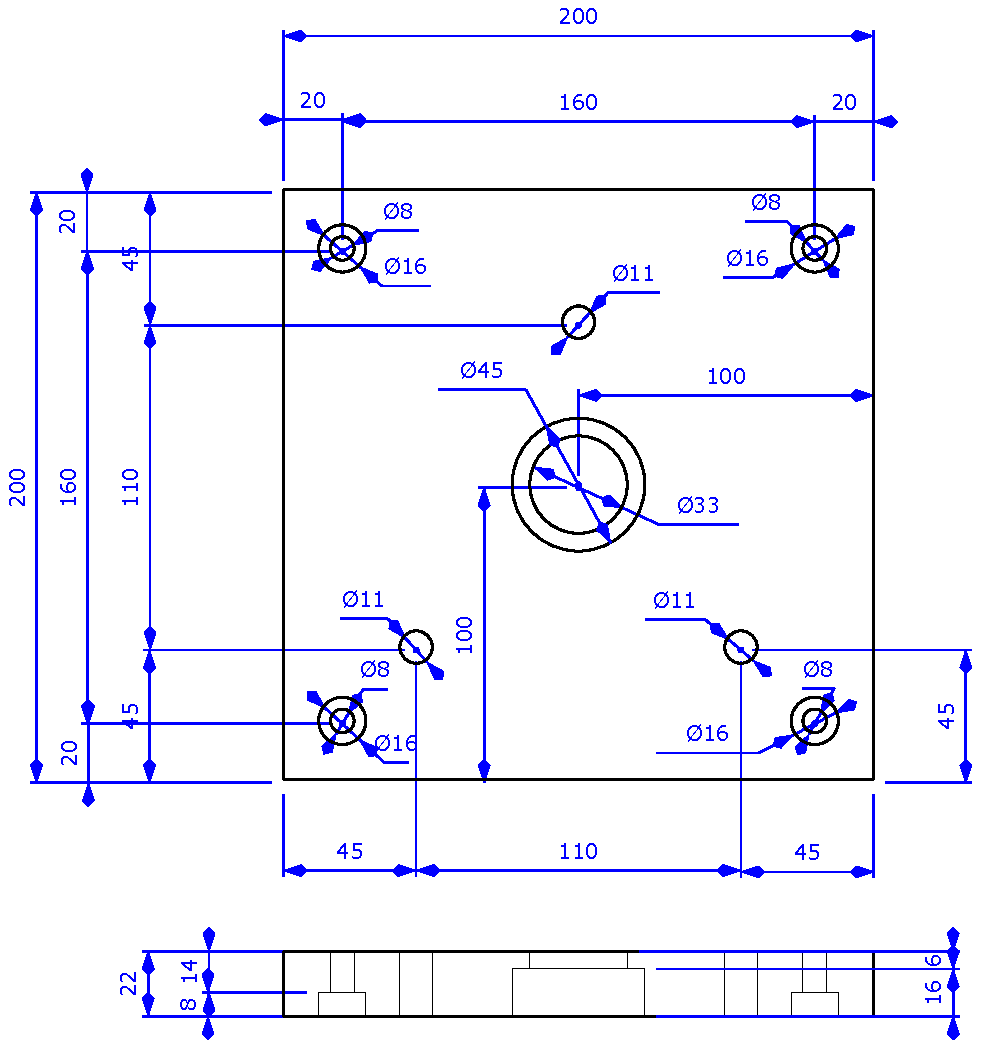
\includegraphics[scale=0.4]{RBR_mod_Bottom}}
  \caption{The top and bottom baffles of the RBR module in scale 1:5}
  \label{fig:appendix-blueprint-rbr-module}
\end{figure}

\begin{figure}[H]
    \centering
    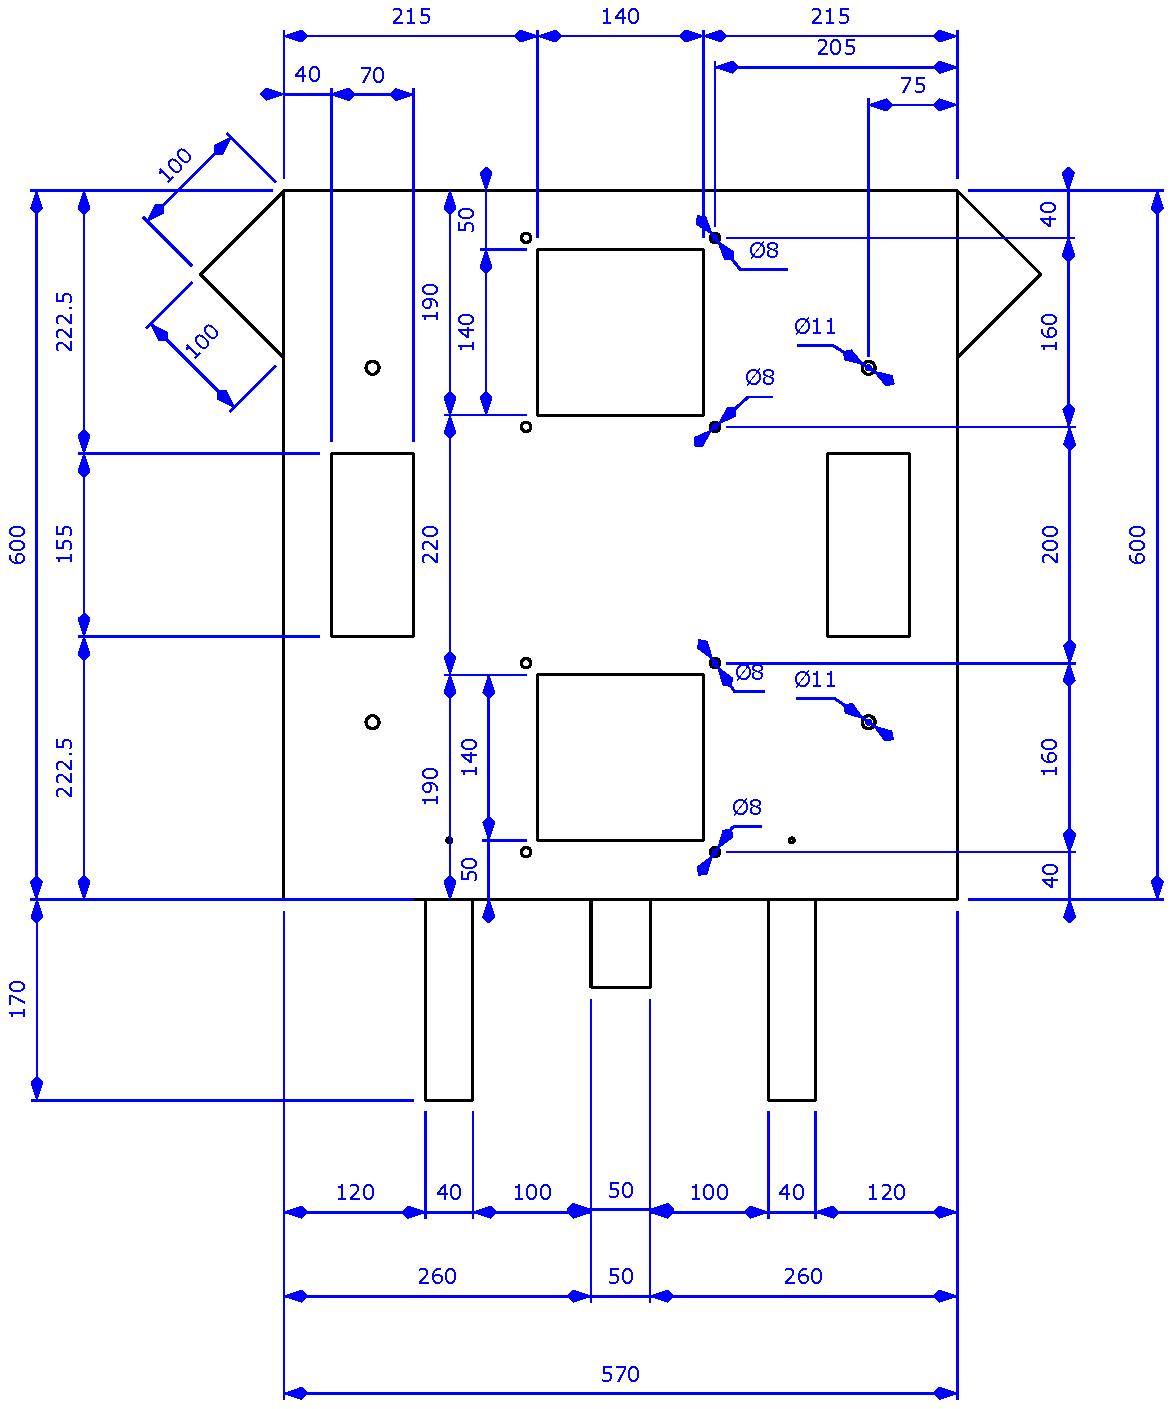
\includegraphics[scale=0.5]{mainPlate}
    \caption{The blueprint of the main baffle in scale 1:10}
    \label{fig:appendix-blueprint-main-plate}
\end{figure}

\begin{figure}[H]
    \centering
    \raisebox{-\height}{ 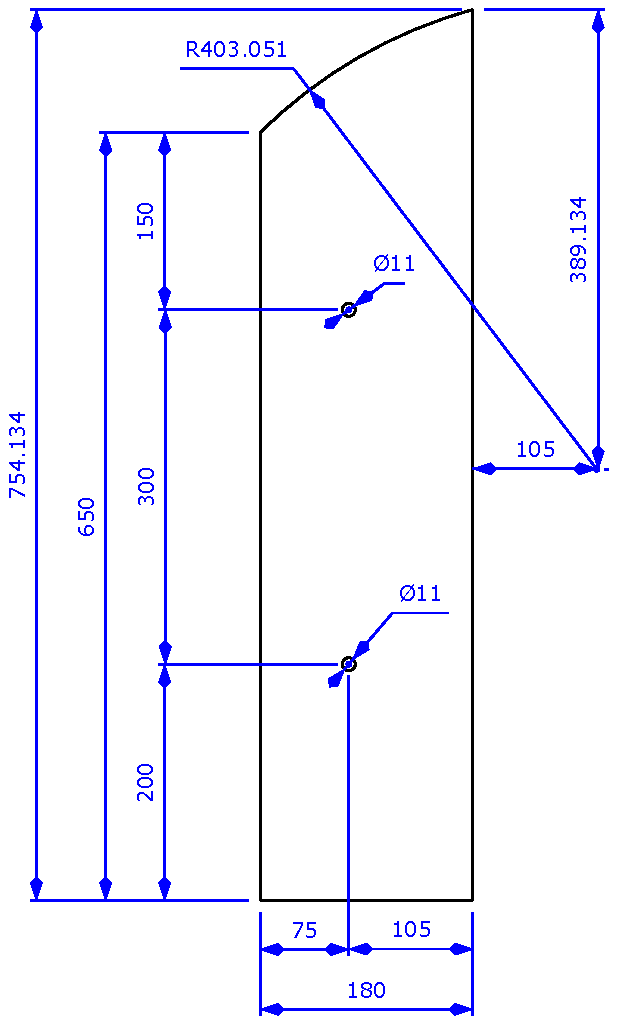
\includegraphics[scale=0.5]{ponton}}
    \raisebox{-1.1\height}{ 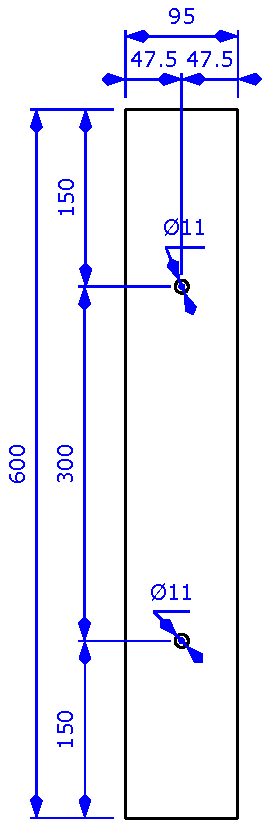
\includegraphics[scale=0.5]{bottom_plank}}
    \caption{The blueprint of one pontoon and the bottom board in scale 1:10}
    \label{fig:appendix-blueprint-ponton}
\end{figure}

\clearpage
\section{Specification of requirements}\label{kravspec}
The following is a translation from the original specification of requirements.

\begin{enumerate}    
    \item One or more RBRs with related equipment must be kept afloat by a vehicle which must meet in order of priority:
    \begin{enumerate}
        \item Withstand rain and waves of up to two inches without compromising function
        \item Evaluate whether the RBRs should be able to move to different depths. Depending on the evaluation this should also be implemented.
        \item The dimensions of the vehicle must be kept in 60x60~cm. No restrictions on the maximum depth.
    \end{enumerate}
    \item Propulsion system for vehicle must meet in order of priority:
    \begin{enumerate}
        \item Only use electric power
        \item Remote control via e.g. radio control
        \item Be useful with one or many RBRs are used
        \item Be constructed such that it is easy to recharge the power source
        \item It should be easy to make the vehicle autonomous at a later stage
        \item Withstand rain (We should be able to overturn the vehicle that the propulsion system is connected to without it breaking.)
    \end{enumerate}
    \item The final product should be simple to use, and so simply designed that it is possible to produce a copy without any major obstacles. This requires drawings and wiring diagrams.
    \item The final product should be built in such a way that it is easy to replace reactants in the RBRs.
    \item The following materials should be tested to see how well they capture the copper and zinc in an aqueous solution using the RBRs. (This will be used as an indicator of how well they purify heavy metals.)
    \begin{enumerate}
        \item Ion exchangers
        \item Zeolites
        \item Concrete
        \item Goethite
        \item Active carbon
    \end{enumerate}
    \item We should produce a final film test which can be used to demonstrate the effectiveness of our solution by reducing the pH of a solution of sodium hydroxide with the product, as well as demonstrate purification using phenolphthalein.
    \item Animation, film or photos to be developed for marketing purposes to show how the end product is used, and in an attractive way present the positives of the product.
\end{enumerate}

\newpage
    \section{Source code}
    Included below are the source code used on the arduino to drive the RBR motor shield.

\subsection{RBR\_driver/RBR\_driver.ino}
The main script controlling the RBR motors.
\lstinputlisting[language=c++]{./RBR_driver/RBR_driver.ino}
\subsection{RBR\_driver/DualVNH5019MotorShield.h}
The h file used taken from \url{https://github.com/pololu/dual-vnh5019-motor-shield} \lstinputlisting[language=c++]{./RBR_driver/DualVNH5019MotorShield.h} 
\subsection{RBR\_driver/DualVNH5019MotorShield.cpp}
The c++ file taken from \url{https://github.com/pololu/dual-vnh5019-motor-shield}
\lstinputlisting[language=c++]{./RBR_driver/DualVNH5019MotorShield.cpp}



%%% Local Variables: 
%%% mode: latex
%%% TeX-master: "document"
%%% End: 

